\documentclass[runningheads]{llncs}

% \usepackage[utf8]{inputenc} % allow utf-8 input
% \usepackage[T1]{fontenc}    % use 8-bit T1 fonts
\usepackage{hyperref}       % hyperlinks
\usepackage{url}            % simple URL typesetting
\usepackage{booktabs}       % professional-quality tables
\usepackage{amsfonts}       % blackboard math symbols
\usepackage{nicefrac}       % compact symbols for 1/2, etc.
\usepackage{microtype}      % microtypography
\usepackage{lipsum}
\usepackage[dvipsnames]{xcolor}
\usepackage{csquotes}
% \usepackage{times}
\usepackage{epsfig}
\usepackage{graphicx}
\graphicspath{{./images/}}
\usepackage{amsmath}
\usepackage{amssymb}
\usepackage{makecell}
\usepackage{diagbox}

\usepackage{comment}

\usepackage{multirow}
\usepackage{bm}
\usepackage{caption}
\captionsetup[table]{position=bottom} 

\let\proof\relax
\let\endproof\relax
\usepackage{amsthm}
\newtheorem{thm}{Theorem}
\newtheorem{defn}{Definition}
\newcommand{\defnautorefname}{Definition}
\newtheorem{lem}{Lemma}
\newcommand{\thmautorefname}{Theorem}
\newtheorem{cor}{Corollary}
\newcommand{\corautorefname}{Corollary}

\newtheorem{prop}{Proposition}
\newcommand{\propautorefname}{Proposition}

\def\ourmodel{\textit{IRAE}}

% ZQ package and command
\usepackage{bbding}
\usepackage{pifont}
\usepackage{wasysym}
\usepackage{amssymb}
\newcommand{\xmark}{\ding{55}}%
\usepackage{tablefootnote}
\usepackage{authblk}
\usepackage{tabularx} 
\usepackage[misc]{ifsym}

\newcommand{\etal}{\textit{et al}. }
\newcommand{\ie}{\textit{i}.\textit{e}., }
\newcommand{\eg}{\textit{e}.\textit{g}. }

\makeatletter
\newcommand{\printfnsymbol}[1]{%
  \textsuperscript{\@fnsymbol{#1}}%
}
\makeatother

% DW package and command
% once we've finished writing we can simply modify this command to keep the latest version.
\newcommand{\rev}[2]{{\color{red}{#1}}$\rightarrow${\color{blue}{#2}}}
\usepackage[normalem]{ulem}
\newcommand{\remove}[1]{\sout{#1}}

\newcommand{\x}{\mathbf{x}}
\newcommand{\y}{\mathbf{y}}
\newcommand{\X}{\mathbf{X}}
\newcommand{\z}{\mathbf{z}}
\newcommand{\m}{\mathbf{m}}
\newcommand{\n}{\mathbf{n}}
\newcommand{\nphi}{n_{\mathbf{\phi}}}
\newcommand{\mii}{\mathbb{I}}
\newcommand{\miiphi}{\mathbb{I}_{\mathbf{\phi}}}
\newcommand{\miin}{\widehat{\mathbb{I}}_{n}}
\newcommand{\ejxy}{\mathbb{E}_{(\mathbf{X},Y)}}
\newcommand{\e}{\mathbb{E}}
\newcommand{\emxy}{\mathbb{E}_{\mathbf{X}}\mathbb{E}_{Y}}
\newcommand{\ejxyn}{\mathbb{E}_{(\mathbf{X},Y)_n}}
\newcommand{\emxyn}{\mathbb{E}_{\mathbf{X}_n}\mathbb{E}_{Y_n}}
\newcommand{\ex}{\mathbb{E}_{\mathbf{X}}}
\newcommand{\ey}{\mathbb{E}_{Y}}
\newcommand{\exn}{\mathbb{E}_{\mathbf{X}_n}}
\newcommand{\eyn}{\mathbb{E}_{Y_n}}

\DeclareMathOperator{\PMI}{PMI}
\DeclareMathOperator{\Diff}{Diff}

\newcommand{\STAB}[1]{\begin{tabular}{@{}c@{}}#1\end{tabular}}

% Include other packages here, before hyperref.
\usepackage{subcaption}
\usepackage{float}

\begin{document}


%%%%%%%%% TITLE


\title{A Stable Training Pipeline for Cascade Networks}

%
%\titlerunning{Abbreviated paper title}
% If the paper title is too long for the running head, you can set
% an abbreviated paper title here
%
\author{Jieli Zheng\inst{1} \and
Zhenyue Qin\inst{1} \and
Yang Liu\inst{1,2}}
%
\authorrunning{JL. Zheng et al.}
% First names are abbreviated in the running head.
% If there are more than two authors, 'et al.' is used.
%
\institute{
Australian National University$^1$, Data61-CSIRO$^2$ \\
% Australian National University, Australia \\
}
%
\maketitle              % typeset the header of the contribution
\email{u6579712@anu.edu.au, yang.liu3@anu.edu.au, zhenyue.qin@anu.edu.au
% , tom@cs.anu.edu.au 
\\} 




%%%%%%%%% ABSTRACT
\begin{abstract}
   The Constructive Cascade Networks~\cite{GeneralisationConstructiveCascade2009} are flexible and expressive deep learning algorithms especially on real-world complex tasks. However, they can suffer from performance drop after modifying the architecture of the network during training. Therefore, in this article we propose a improved training pipeline for Casper Network~\cite{CascadeCorrelation1990}, Conditional VAE-Casper algorithm to classify several real-world diseases by few physiological indicators and analyse the stable performance of CVAE-Casper during training. We will give out experimental results and analyse the improvements compared to the vanilla Casper Network, the advantages and drawbacks of CVAE-Casper. Finally, We will talk about the possible improvements of CVAE-Casper to explore future works.

\end{abstract}

%%%%%%%% KEYWORDS
\keywords{Computer Science  \and Artificial Intelligence \and Classification \and Cascade networks \and Constructive networks \and Casper.}

%%%%%%%% Introduction 
\section{Introduction}
The deep neural network has got unparalleled success in Artificial Intelligence due to its generalization ability. Pre-defined network architecture and hyper-parameters are necessary before training classic neural networks algorithms, and the performance of neural networks like CNN are usually sensitive to these settings~\cite{CNNClassification2015}. Constructive model is a good way of estimate the problem complexity by the network complexity which is computationally economical~\cite{constructive}. However, constructive networks usually make use of greedy approach to find an appropriate network architecture~\cite{constructive}, the performance of the model may drop right after adding new initialised neurons. In this article we intend to use a modified version of Constructive Cascade Networks ~\cite{GeneralisationConstructiveCascade2009}, Generative Cascade Network Employing Progressive RPROP, or CVAE-Casper ~\cite{CASPER1997} which is inspired by ~\cite{CASPER1997} and ~\cite{cvae}, to solve two medical classification problem, and show that CVAE-Casper has more stable performance than vanilla Casper while training. \\
There are two datasets to validate our work. The first one is SARS-CoV-1 dataset. SARS-CoV-2, also known as COVID-19, has become a global pandemic disease from 2020 spring and also a landmark event in history. For the first dataset we are intended to build a classification deep learning model on the first SARS subspecies: SARS-CoV, which has more severe symptoms, higher fatality rate and lower transmission rate ~\cite{SARSCOV2_2020}. Since some physiological indicators like sequential body temperature are easy to measure, we will only use sequential body temperature for classification task. The secondly dataset is Cardiovascular disease dataset. The second classification task is more complex than the first one and the model will make use of physical examination data to predict Cardiovascular disease. We will analyze the stability of CVAE-Casper under both simple and complex dataset. The contributions we made in this article are as follows. Firstly, we introduced a new training method for constructive cascade network to both obtain stable performance while training and higher test accuracy while testing. Secondly, we introduced two classification model that can well predict SARS and Cardiovascular diseases which are common now.

%%%%%%%% Related Work 
\section{Related Work}
Constructive Networks are a type of neural network which can modify their architecture while training. Cascade correlation Network was introduced in 1990 ~\cite{CascadeCorrelation1990}. The constructive architecture was designed to extract features by adding correlated neurons. Since the hidden neurons have weights frozen once added, the performance may be bad due to early poor neurons~\cite{CASPER1997}. Casper was introduced to solve this by setting leaky learning rate for frozen weights. However, both Cascade correlation and Casper network still suffer from accuracy drops while adding neurons. In this article a new training pipeline is introduced to improve the training loss while training and the final test results.

%%%%%%%% Preliminaries Approaches
\section{Approaches}
\subsection{Casper Network Topology}
Constructive neural networks are constructive because they will change the architecture of themselves when loss is no longer improved. Here firstly Casper networks start as a simple fully connected network with only input and output layer in Fig.1.1. It’s obvious that such a vanilla fully connected one-layer neuron network is usually not expressive enough to extract the features in training data. Once the loss is non-decreasing, the Casper will add a new neuron into the network. Compared to Cascor, Casper will not freeze previous additional neurons and set difference learning rate to each weight. In Fig.1.2, we can see the difference of each learning rate: L1, L2 and L3. Generally, the value of L1, L2 and L3 are 0.2, 0.005 and 0.001 referring to the technique paper. Learning rate of weights connected to the latest neuron will be set to L1 since the latest neuron is expected to be the feature extractor, and a larger learning rate can speed up the feature learning process. Similarly, the new extracted feature output should reduce the loss without too much interference from the previous weights ~\cite{CascadeCorrelation1990}. Hence it should be set to L2 which is slightly larger than the L3. Since no neurons are frozen, the previous neurons can still be modified if it’s necessary and beneficial. Then the model can both obtain the benefit of the weight freezing and the correlation techniques of Cascor, while avoiding early poor hidden neurons due to weight freezing and the saturation problems due to correlation measure. ~\cite{vae2020}\\

\begin{figure}[hbt!]
\centering
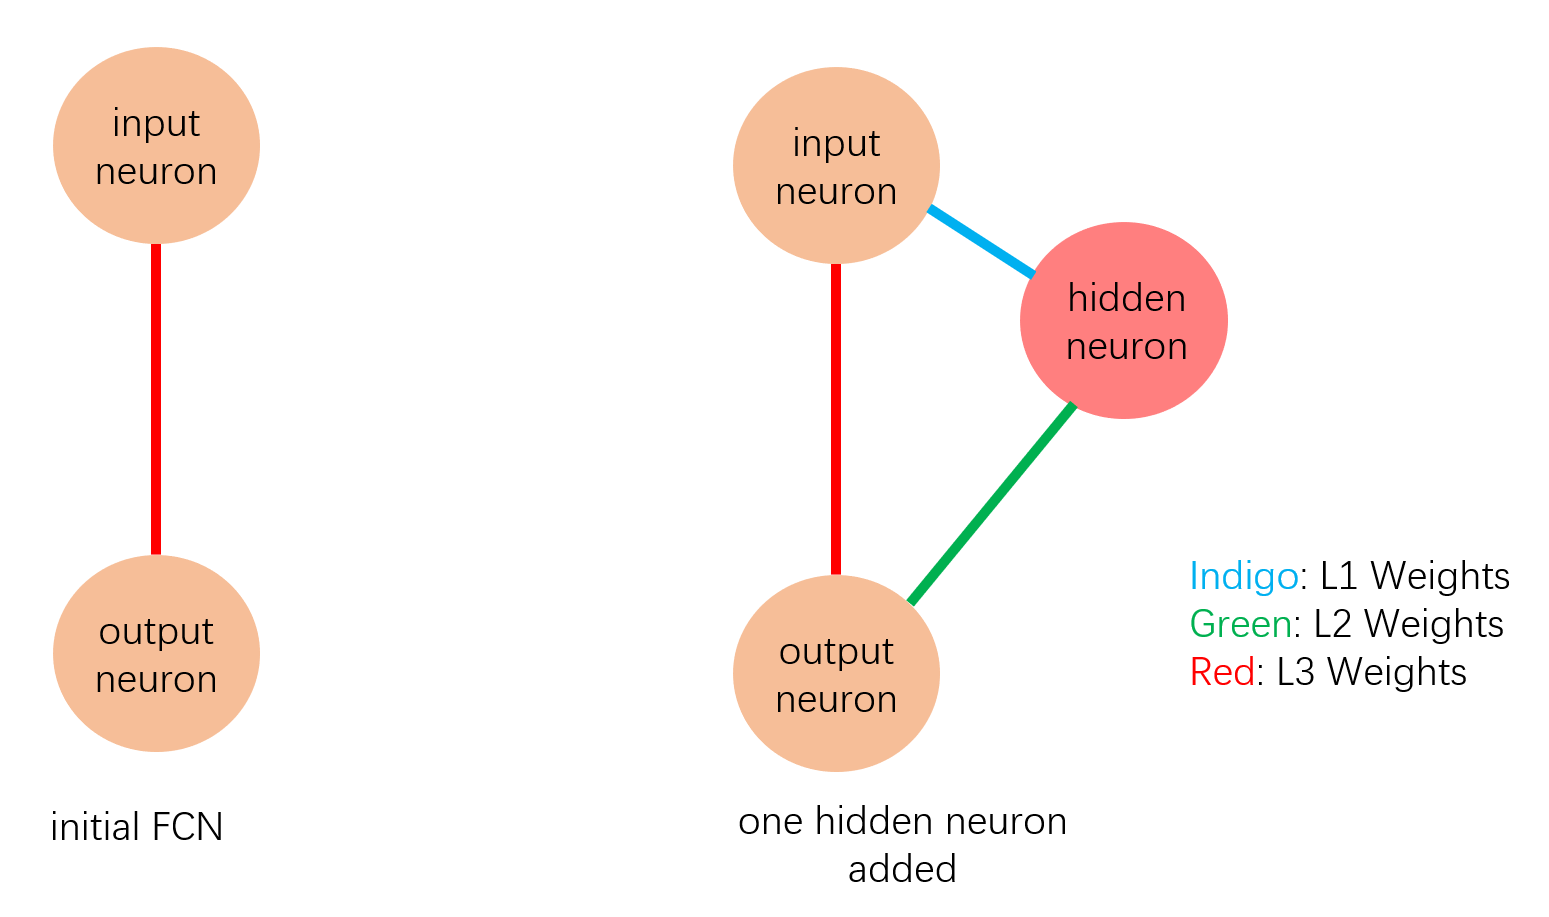
\includegraphics[width=\textwidth]{images/reimg1.png}
\caption{The process to add a random hidden neuron into the network}
\label{figure1}  
\end{figure}

As is shown above in Fig2., it is almost the same when the model add another neuron into the network. Input neuron to 2nd hidden neuron and 1st hidden neuron to the 2nd hidden neuron use the largest weight to significantly change their value to learn features. L2 learning rate is used for the weight between 2nd hidden neuron to the output neuron, which is the output of the latest neuron and needs to give out a more flexible output than previous outputs. In general, the weights connect between input, the previous hidden neurons and the latest hidden neuron share the largest L1 learning rate, and L2 learning rate is used for the weight connects between the latest hidden neurons to the output, which is larger than L3. Therefore, the rest weights perform L3 weight which is the smallest and difficult to change its state.\\
\begin{figure}[H]
\centering
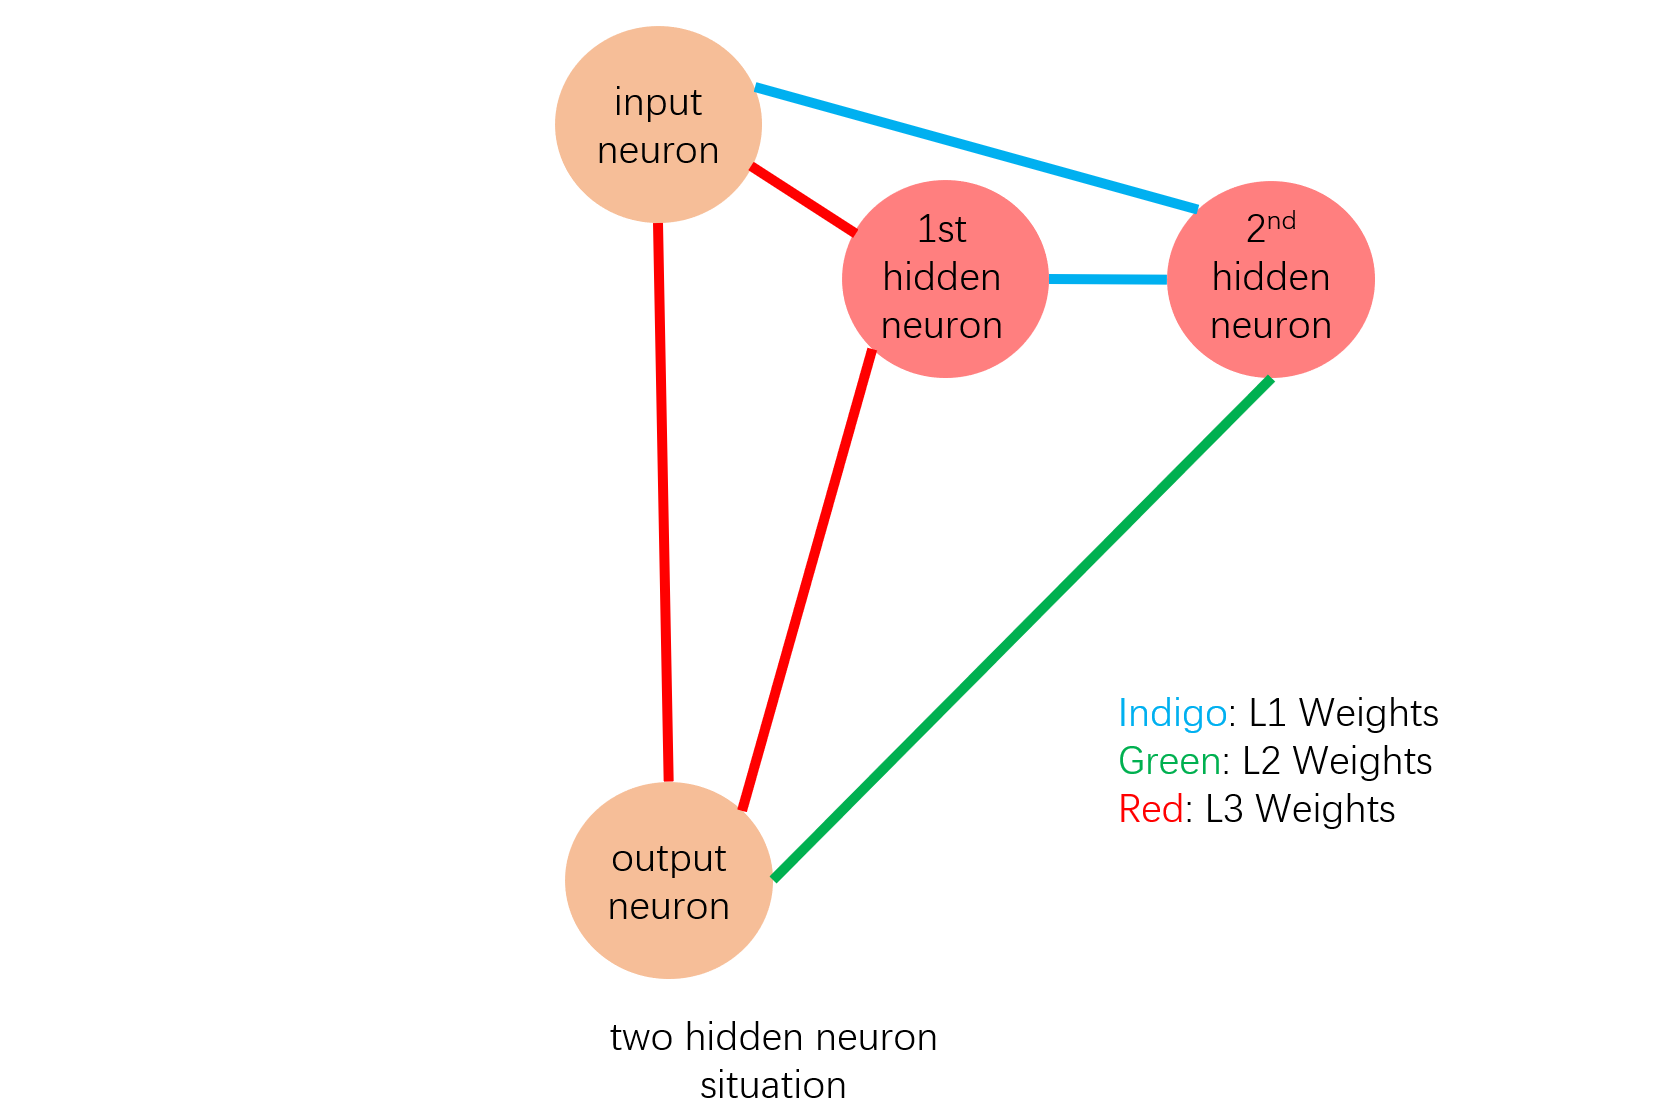
\includegraphics[width=\textwidth]{images/reimg2.png}
\caption{The process to add another hidden neuron}
\label{figure2}  
\end{figure}

\subsection{Conditional Variational AutoEncoder}
AutoEncoder is usually used to find efficient data encodings in an unsupervised manner. Variational AutoEncoder, or in short VAE, are a subclass of AutoEncoder~\cite{vae2020}. VAE provides a probabilistic manner for describing an observation in latent space. Thus, rather than encode the data to a single vector to compress information, we try to make use of the probability distribution to generate data. Here normal distribution is assumed for the following SARS-CoV Dataset. This is quite beneficial if the raw data has large variance and large dimension. A standard VAE should have the architecture in Fig.3. The data is compressed to its latent vector representation by variational encoder. The major difference between variational encoder and standard encoder is reparametrizing data to find the best mean and variance of latent distributions instead of finding latent representations blindly. Hence the latent vector is sampled from the latent calculated distributions in encoder. Thus, the decoder can sample the latent vector from the latent distributions to reconstruct the original data.\\
\begin{figure}[hbt!]
\centering
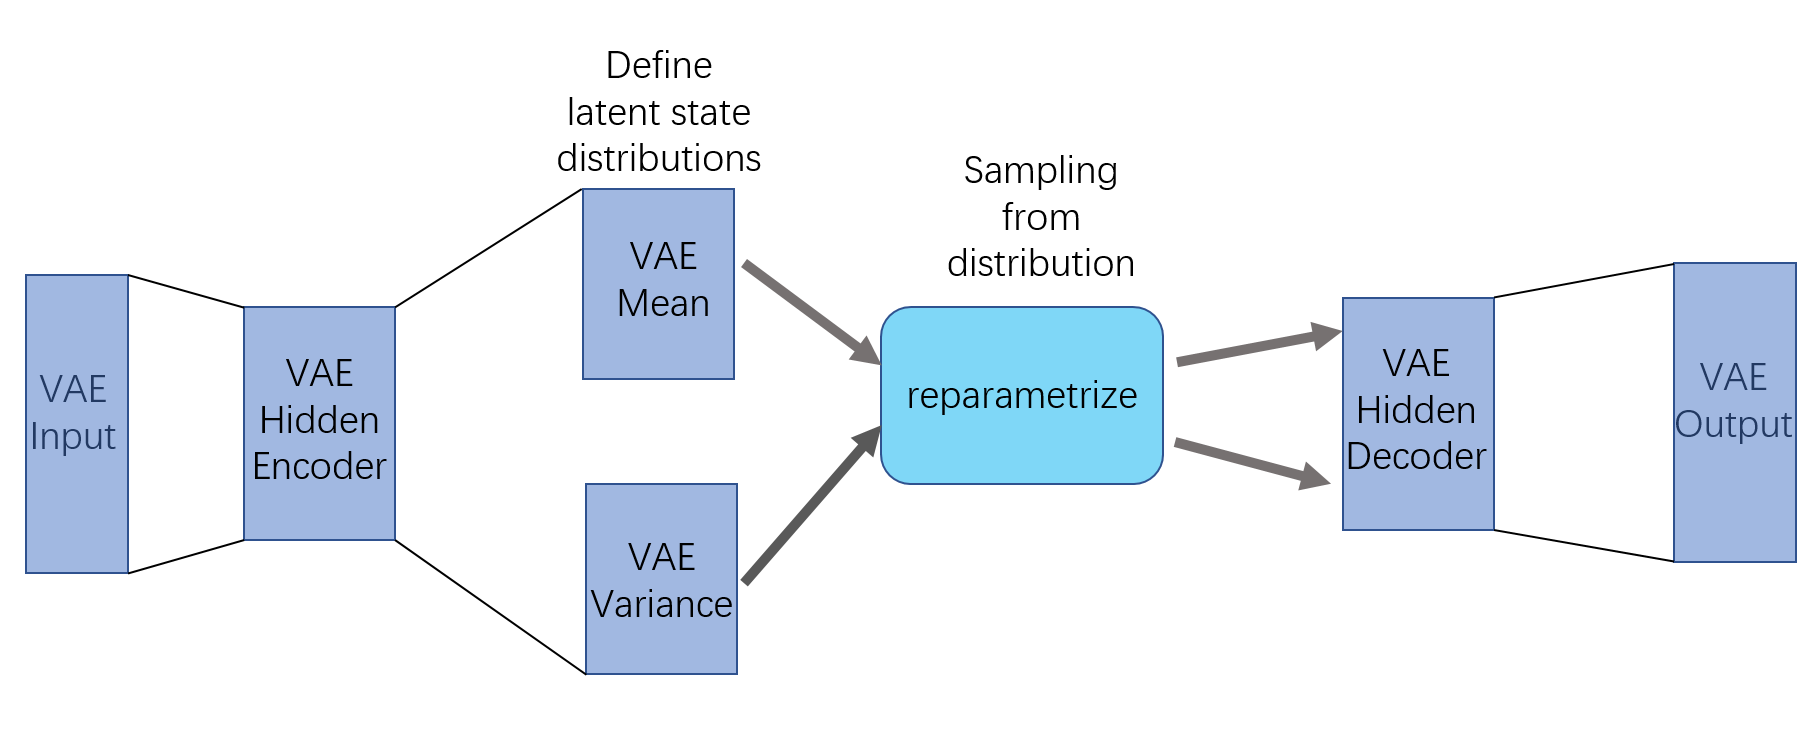
\includegraphics[width=\textwidth]{images/reimg3.png}  
\caption{Vanilla VAE architecture}
\label{figure3}  
\end{figure}

For Conditional VAE ~\cite{cvae}, we can condition the encoder and decoder of VAE to force the model to find different latent space by classes. In other words, we condition all latent distributions with a conditional label $\mathbf{c}$. The conditioning label c is the difference between conditional VAE and vanilla VAE and the latent distribution space becomes: $P(z|c)$ instead of $P(z)$, as the conditional objective is shown below.
$$  
\log P(X \mid c)-D_{K L}[Q(z \mid X, c) \| P(z \mid X, c)]=E[\log P(X \mid z, c)]-D_{K L}[Q(z \mid X, c) \| P(z \mid c)]
$$
\begin{figure}[hbt!]
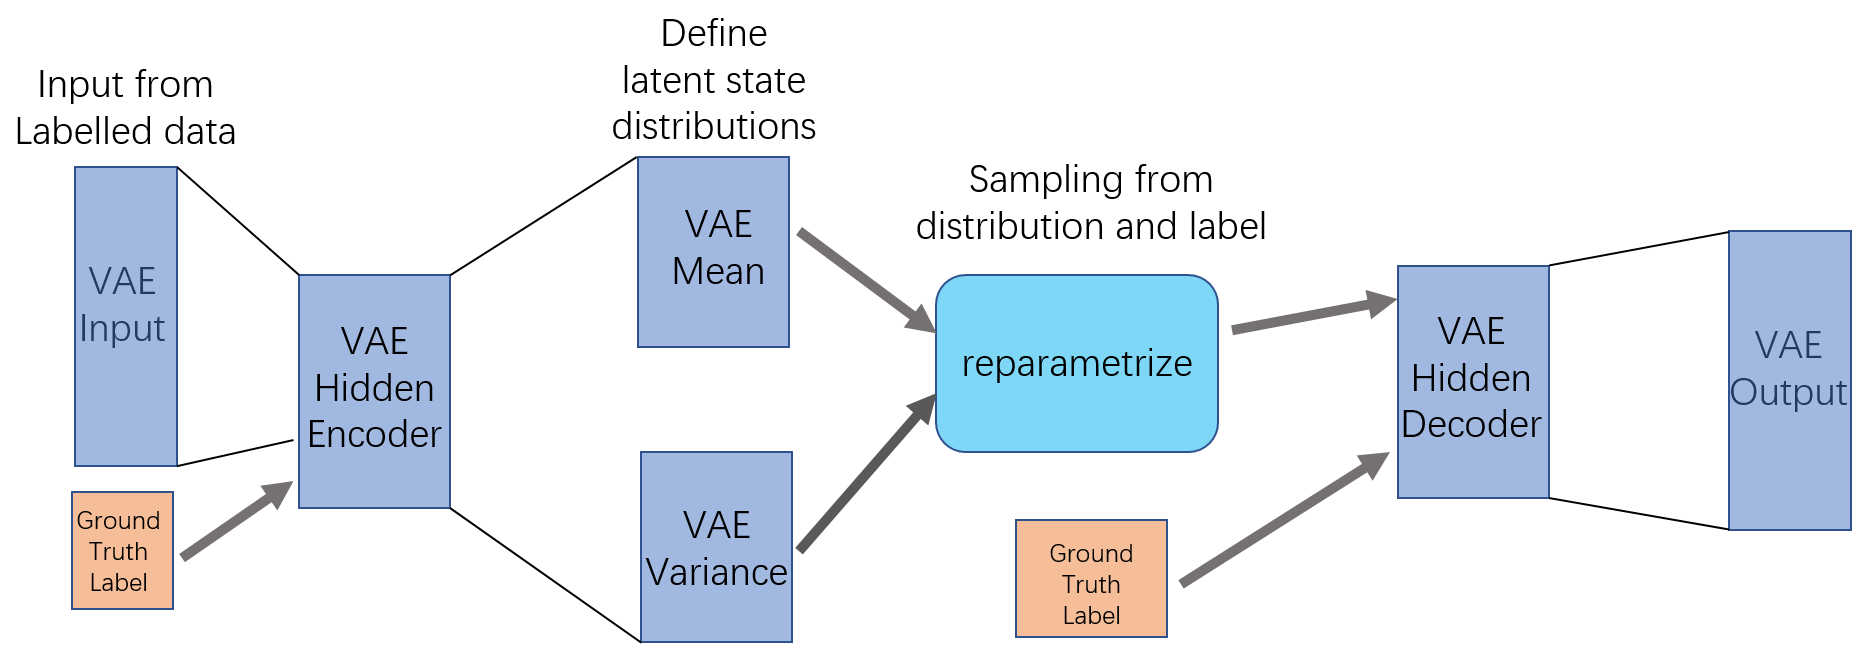
\includegraphics[width=\textwidth]{images/reimg4.png}  
\caption{Conditional VAE architecture}
\label{figure4}  
\end{figure}

Therefore, generative data by conditioning corresponding label can be retrieved from conditional VAE.
\section{Training Pipeline}
The training pipeline we introduce here is as follows. The first module is the CVAE module. Firstly the training data with label is used to train the Conditional VAE module. Since it's Conditional VAE that can generate similar data given labels, we will let CVAE module generates augmentation data given labels we need. Here we choose to generate data four times size larger than the training data. The labels are uniformly distributed while generating. After CVAE comes Casper module, and the Casper makes use of both the original training data and the generated data to train. \\ 
\begin{figure}[H]
\centering
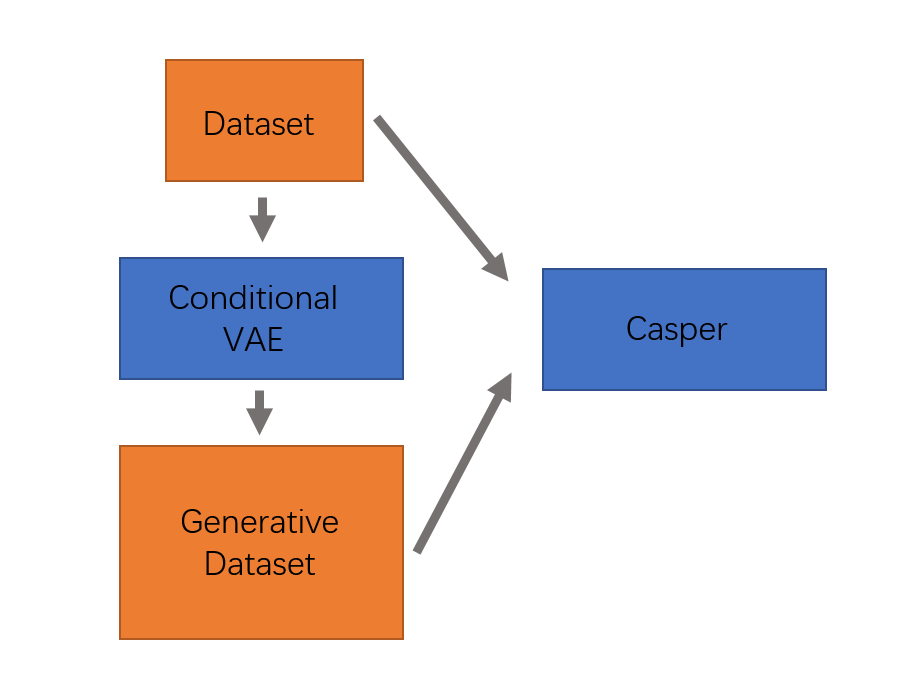
\includegraphics[width=\textwidth]{images/reimg5.png}  
\caption{Training pipeline}
\label{figure5}  
\end{figure}




%%%%%%%% Result & Analysis 
\section{Experimental Results and Analysis}
\subsection{SARS-CoV-1 Dataset}
The first dataset we use for CVAE-Casper Algorithm is SARS-CoV dataset from B. Sumudu U. Mendis1, Tamás D. Gedeon1, László T. Kóczy ~\cite{dataset1_2005}, which is a tiny dataset containing physiological indicator data. One datapoint here is a 23-dimension data, and the range of each element has already been normalized. For example, temperature at 8am has three attributes: slight, medium, high, and they are normalized by default. Also, there isn’t any noise datapoints in the dataset. In SARS-CoV dataset, there are 4000 datapoints for 4 labels: SARS patients, Normal people, High BP patients and Pneumonia patients. Since some of the attributes are so iconic that if some conditions are satisfied, we can directly assert the label of the datapoint, e.g. Only SARS patients have abdominal pain, high body temperature and nausea at the same time. Therefore, this classifier problem will become a linear problem and no need to use neural networks. Also, some physiologic indexes like blood pressure are hard for people to track in daily life. Hence, we try to choose only body temperature by time as the input data. Also, body temperature is significant medical data which are easy to track and highly related to SARS. ~\cite{covidfeatures2020} As a result, the dimension of the input data will be 12 which are sequential body temperatures. A quick peek of the data is as follows.


\begin{table}
\begin{tabular}{|l|l|l|l|l|l|l|l|l|l|l|l|}
\hline
\multicolumn{3}{|l|}{Temp 8am} & \multicolumn{3}{l|}{Temp 12pm} & \multicolumn{3}{l|}{Temp 4pm} & \multicolumn{3}{l|}{Temp 8pm} \\ \hline
       slight&      medium&         high&   slight&      medium&      high&  slight&      medium&      high& slight&   medium& high             \\ \hline
       0.1013&       0.929&       0.842 &       0.0562&  0.7416&  0.6964  &       0&      0.7896&    0.6821&       0&       0.6884&   0.8575    \\ \hline
       0.8827&       0.1286&       0    &       0.9332&       0.0946&   0 &       0.9204& 0.0823&         0&       0.8639&      0.152 &  0     \\ \hline
       1&       0&                     0&       1&       0&              0&               1&       0&     0&       1&       0&       0      \\ \hline
       0.0827&       0.8573&       0.8759&       0.1332&       0.7893&       0.8858& 0.0639& 0.904&  0.8846&       1&       0&       0\\ \hline
\end{tabular}
\caption{A quick peek of SARS-CoV Dataset}
\end{table}





The first task for my previous work ~\cite{selfref2021} is the same as here which is to classify the SARS patients, Pneumonia patients, people with high blood pressure and normal people. Since the dataset is a small sample dataset with 4000 datapoints in total, we expect that choosing 2-layer variational encoder is appropriate for this SARS classification problem. The dimension of the input datapoints is 12 as mentioned before, and the labels use one-hot encoding. We set the number of epochs to 90 to control variables and compare CVAE-Casper to my previous work. The optimizer used here is RMSprop which is the same as described in Casper ~\cite{CASPER1997}, with $momentum=0.9, weight_decay=0.00001, centered=True$. We generate twice larger generative dataset than original training data. The main loss function is the cross-entropy loss function, which is usually for classic classification problems ~\cite{semisupervised2021}. We are intended to use the accuracy on test dataset to evaluate the performance. And The baseline we choose is CasCor from my previous work since the Cascade Correlation is one of the vanilla cascade networks ~\cite{constructive} and CVAE-Casper is a modified version of Casper ~\cite{CASPER1997}, which is a successor architecture of Cascor. The policy of adding neurons for both Cascor and CVAE-Casper is each time the loss does not drop, and use an adding cool-down of 5 epochs to limit the adding frequency of the model. The accuracy and loss chart of CasCor and CVAE-Casper is as follows:
\begin{center}
\begin{tabular}{ c c c }
\hline
 Algorithm & Final Training Loss & Final Test Accuracy \\ 
\hline
 Cascor & 0.472 & 74.351\% \\  
\hline
 CVAE-Casper & 0.004967 & 98\% \\
\hline
\end{tabular}

\end{center}
From the chart above, it’s obvious that CAVE-Casper has dominant performance on SARS-CoV dataset. The final test accuracy is quite high which indicates that the CAVE-Casper can solve more complex problem than SARS classification. Also, the final training loss of CAVE-Casper is close to zero, which indicates that generative Casper can precisely match the problem complexity with the complexity of the neural network and the network should perform early stopping to avoid potential overfitting problem. 

\begin{align*}
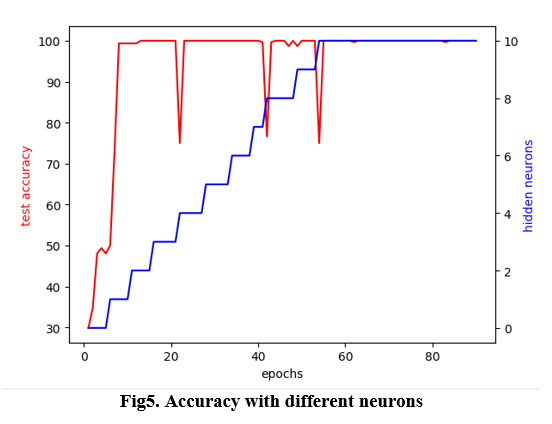
\includegraphics[width=\textwidth]{images/img9.png}
\end{align*}

\begin{align*}
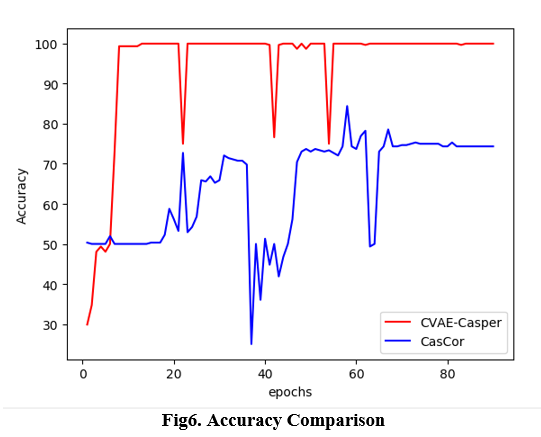
\includegraphics[width=\textwidth /2]{images/img10.png}  
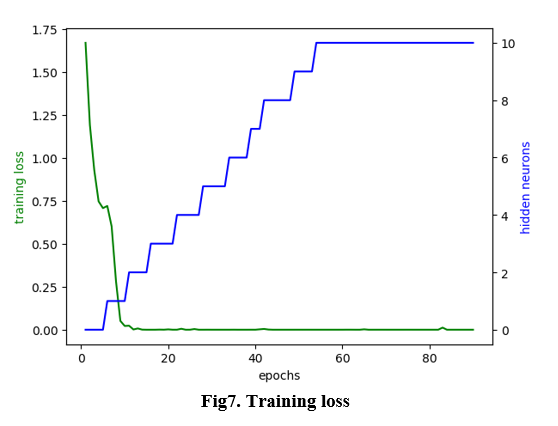
\includegraphics[width=\textwidth /2]{images/img11.png}
\end{align*}

From Fig5 It’s observed that test accuracy of CVAE-Casper rises from 30\% up to 95\% in the first 10 epochs with 2 neurons added. Afterwards, the model quickly finds the global minimum of the loss function in around 15 epochs, where the test accuracy reaches nearly 100\%. Since adding two neurons is enough to get an appropriate 95\% test accuracy, CVAE-Casper is quite strong to solve this problem. If an appropriate termination condition like test accuracy threshold is set for this model to perform early stopping, CVAE-Casper should stop with 2 neurons to achieve a relatively high accuracy. This demonstrates that CVAE-Casper can make use of conditioning to generate high quality data with label to help disease prediction. After the model converges to high test accuracy, we find some performance drops while adding new cascade neurons in epoch 4, 8 and 10, and it quickly adapts and resumes high accuracy since Cascade Correlation networks sometimes face accuracy drop due to newly added neurons are initialized randomly to a bad situation. Fig6 contains the accuracy comparison between CasCor and CVAE-Casper. There are several reasons for the dominant performance of CVAE-Casper compared to CasCor. First of all, vanilla Casper does not freeze any previous added neuron, and CasCor may freeze poor feature extractors which is difficult for output weight to adjust their poor features. Since the algorithm still allows the previous poor hidden neurons to update their input weights by a small learning rate (L3), the poor neurons still have chance to update themselves. Secondly, the original dataset is small and CVAE-Casper is able to generate more data from conditioning to help the classification task. Thirdly, according to Gedeon, T. D. (1997)~\cite{CASPER1997}, Casper can resume the property of CasCor that the latest neurons are the latest feature extractors since the learning rate of the previous hidden neurons is small with respect to the learning rate (L1) of the latest hidden neurons.






\subsection{Cardiovascular Disease Dataset}
The second dataset we use for CVAE-Casper is a Cardiovascular disease dataset from Kaggle open dataset\footnote{Retrieved from Kaggle: https://www.kaggle.com/sulianova/cardiovascular-disease-dataset}, which is a much larger dataset with physiological data. Each datapoint contains several medical indicator including: height, weight, Systolic blood pressure, Diastolic blood pressure, cholesterol, gluc, BMI, age and smoke to predict whether the patient has potential Cardiovascular Disease. The size of the dataset is 70,000 and the classes are well balanced between Cardiovascular Disease case and normal people. We are using this dataset to verify that CVAE-Casper has stable performance among various medical datasets.


\begin{table}[]
\begin{tabular}{|l|l|l|l|l|l|l|l|l|l|l|l|}
\hline
age & gender & height & weight & Systolic BP & Diastolic BP & cholesterol & gluc & smoke & alco & active & cardio(Label) \\ \hline
18393 & 2 & 168 & 62.0 & 110 & 80  & 1 & 1 & 0 & 0 & 1 & 0 \\ \hline
20228 & 1 & 156 & 85.0 & 140 & 90  & 3 & 1 & 0 & 0 & 1 & 1 \\ \hline
18857 & 1 & 165 & 64.0 & 130 & 70  & 3 & 1 & 0 & 0 & 0 & 1 \\ \hline
17623 & 2 & 169 & 82.0 & 150 & 100 & 1 & 1 & 0 & 0 & 1 & 1 \\ \hline
\end{tabular}
\caption{A quick peek of Cardiovascular Dataset}
\end{table}



The second dataset is aimed to find that conditional VAE is beneficial to consistent performance. The task here is to predict whether the given patient has Cardiovascular disease, which is a binary classification problem. The optimizer,encoding and the epochs are the same as the first experiment. Since it's a classification problem, cross-entropy loss is still used here.  The generative data is 100,000, which is much larger than the original training data(70,000). The baseline we choose is the vanilla Casper~\cite{CASPER1997} since we will analyze whether the CVAE generated data can avoid or improve the performance drop in Casper.

\begin{center}
\begin{tabular}{ c c c }
\hline
 Algorithm & Final Training Loss & Final Test Accuracy \\ 
\hline
 Casper & 0.75635 & 64.56\% \\  
\hline
 CVAE-Casper & 0.63835 & 68.69\% \\
\hline
\end{tabular}
\end{center}
From the chart above, the final test accuracy is around 5\% higher than the vanilla Casper. CVAE-Casper and vanilla Casper both uses 10 neurons to achieve such results. As a result, the CVAE-Casper has an edge over vanilla Casper due to its conditioning generative data. As detailed figures are as below.

\begin{align*}
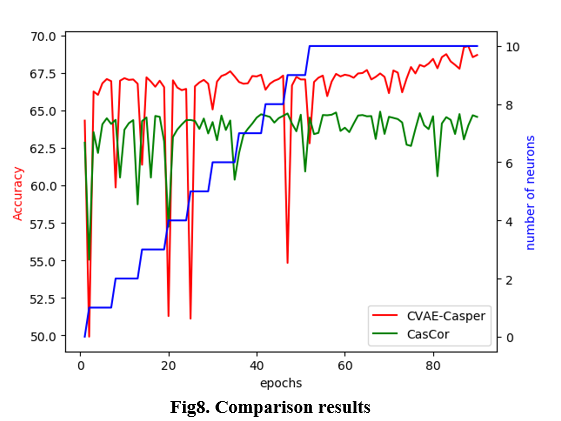
\includegraphics[width=\textwidth]{images/img12.png}
\end{align*}
From Fig8 it's observed that CVAE-Casper has better test accuracy during all training epochs except for several epochs that new random neuron is added into the architecture. Since the training set after adding generative data is much larger than the original dataset, it's expected that the random neuron is affected more by the large generative training set and the loss will be higher.

%%%%%%%% Conclusion & Future Work 
\input{components/con}





% \clearpage
{\small
\bibliographystyle{splncs04}
% \bibliography{egbib}

\begin{thebibliography}{10}
\providecommand{\url}[1]{\texttt{#1}}
\providecommand{\urlprefix}{URL }
\providecommand{\doi}[1]{https://doi.org/#1}

\bibitem{CascadeCorrelation1990}
Fahlman, S.E., and Lebiere, C. (1990) The cascade-correlation learning architecture. 
In Advances in Neural Information Processing II,Touretzky, Ed. SanMateo, CA: Morgan 
Kauffman, 1990, pp. 524-532.

\bibitem{GeneralisationConstructiveCascade2009}
Khoo S., Gedeon T. (2009) Generalisation Performance vs. Architecture Variations in Constructive Cascade Networks. In: Köppen M., Kasabov N., Coghill G. (eds) Advances in Neuro-Information Processing. ICONIP 2008. Lecture Notes in Computer Science, vol 5507. Springer, Berlin, Heidelberg. \doi{10.1007/978-3-642-03040-6_29}

\bibitem{CNNClassification2015}
Zhang, Y., \& Wallace, B. (2015). A sensitivity analysis of (and practitioners' guide to) convolutional neural networks for sentence classification. arXiv preprint arXiv:1510.03820.

\bibitem{SARSCOV2_2020}
Eskild, P., Marion, K., Unyeong, G., Davidson, H, H., Nicola, P., Francesco, C., Merete, S., Sulien, Al, K., Lone, Simonsen. (2020). Comparing SARS-CoV-2 with SARS-CoV and influenza pandemics. The Lancet Infectious Diseases, 20, 238-244. Retrieved April 24, 2021, from \doi{10.1016/S1473-3099(20)30484-9}


\bibitem{CASPER1997}
Treadgold, N. K., \& Gedeon, T. D. (1997, June). A cascade network algorithm employing progressive RPROP. In International Work-Conference on Artificial Neural Networks (pp. 733-742). Springer, Berlin, Heidelberg.

\bibitem{variationscascade1998}
Treadgold, N. K., \& Gedeon, T. D. (1998, May). Exploring architecture variations in constructive cascade networks. In Neural Networks Proceedings, 1998. IEEE World Congress on Computational Intelligence. The 1998 IEEE International Joint Conference on (Vol. 1, pp. 343-348). IEEE.

\bibitem{exploringcascade1999}
Treadgold, N. K., \& Gedeon, T. D. (1999). Exploring constructive cascade networks. IEEE Transactions on Neural Networks, 10(6), 1335-1350.

\bibitem{dataset1_2005}
Mendis, B. S., Gedeon, T. D., \& Koczy, L. T. (2005). Investigation of aggregation in fuzzy signatures, in Proceedings, 3rd International Conference on Computational Intelligence, Robotics and Autonomous Systems, Singapore.  \url{http://users.cecs.anu.edu.au/~Tom.Gedeon/pdfs/Investigation%20of%20Aggregation%20in%20Fuzzy%20Signatures.pdf}

\bibitem{covidfeatures2020}
Huang, C., Wang, Y., Li, X., Ren, L., Zhao, J., Hu, Y., Zhang, L., Fan, G., Xu, J., Gu, X., Cheng, Z., Yu, T., Xia, J., Wei, Y., Wu, W., Xie, X., Yin, W., Li, H., Liu, M., . . . Cao, B. (2020). Clinical features of patients infected with 2019 novel coronavirus in wuhan, china. The Lancet (British Edition), 395(10223), 497-506. \doi{10.1016/S0140-6736(20)30183-5}


\bibitem{transferlearning2018}
Gao, Y., \& Mosalam, K. M. (2018). Deep transfer learning for Image‐Based structural damage recognition. Computer-Aided Civil and Infrastructure Engineering, 33(9), 748-768. \doi{10.1111/mice.12363}


\bibitem{vae2020}
Weonyoung Joo, Wonsung Lee, Sungrae Park, Il-Chul Moon, Dirichlet Variational Autoencoder, Pattern Recognition,
 Volume 107, 2020, 107514, ISSN 0031-3203, \doi{10.1016/j.patcog.2020.107514}.
 
 \bibitem{vae2018}
Jeremy Jordan. (2018). Variational autoencoders. Retrieved from \url{https://www.jeremyjordan.me/variational- autoencoders/}

\bibitem{selfref2021}
Zheng, J (2021) Best match between SARS classification and Constructive Correlation Neuron Networks, ABCs 2021 

\bibitem{semisupervised2021}
Lima, B. V. A., Neto, A. D. D., Silva, L. E. S., \& Machado, V. P. (2021). Deep semi‐supervised classification based in deep clustering and cross‐entropy. International Journal of Intelligent Systems, \doi{10.1002/int.22446}

\bibitem{cvae}
Ruichen, ZHANG, et al. "Widespread Bathymetric Outliers Detection and Elimination Based on Conditional Variational Autoencoder Generative Adversarial Network." Ce Hui Xue Bao, vol. 48, no. 9, 2019, pp. 1182-1189


\bibitem{constructive}
Kwok, Tin-Yau \& Yeung, Dit-Yan. (1997). Constructive algorithms for structure learning in feedforward neural networks for regression problems. Neural Networks, IEEE Transactions on. 8. 630 - 645. 10.1109/72.572102. 

\bibitem{cvaeimage}
Isaac Dykeman (2016). Conditional Variational Autoencoders. Retrieved from \url{https://ijdykeman.github.io/ml/2016/12/21/cvae.html}

\bibitem{pastConstructive}
Sharma, Sudhir & Chandra, Pravin. (2010). CONSTRUCTIVE NEURAL NETWORKS: A REVIEW. International Journal of Engineering Science and Technology. 2. 


\end{thebibliography}

}


% \newpage
% \onecolumn
% \appendix
% \input{secs/supplementary.tex}

\end{document}
